\chapter{Introduction}

% Introduction: the paper's objectives and short description of chapters, overview of theme, highlight of personal contribution versus original results, and mention (if applicable) of the communication session where it was presented or the journal where it was published.

\section{Context}

With the rise of mobile devices, users are now able to access many different services directly from their phones. Companies and government agencies are constantly digitizing themselves, and offering their services on mobile devices proves to be the easiest method of reaching their users.

However, methods of delivering applications on mobile phones differ greatly, from phone vendor to another, but also within vendors. Each phone manufacturer provides their own custom way of creating applications for their operating system (Android, iOS). A large-scale study by Haipeng Cai et. al. shows \cite{HaipengAndroidIncomp} that even within Android-based phones exist different flavors of operating systems (by Google, Huawei, Samsung) that are pose incompatibilities to apps, in subtle ways.

As time progressed and the Web evolved, a novel way of creating web applications, that was sitting right on the bridge between native apps and website-based applications, started to form. Starting as early as the year 2000, \verb|XMLHttpRequest| was available on Microsoft's Internet Explorer, and AJAX happened five years later. These, among others, proved to be key parts of the new architecture that designer Frances Berriman and Google engineer Alex Russell coined as "progressive web apps", back in 2015 \cite{PWAShortHist}.

These Progressive Web Apps would advertise themselves as such by using a "web app manifest", and they could register a "service worker" with the browser to put control of the browser's request-response lifecycle in the app's hands \cite{WHATWGWorkers}.

The PWA architecture is described in Alex Russell's words using the following attributes: \cite{PWAShortHist}
\begin{itemize}
    \item \textbf{Responsive:} to fit any form factor;
    \item \textbf{Connectivity independent:} progressively-enhanced with Service Workers to let them work offline;
    \item \textbf{App-like-interactions:} adopt a shell + content application model to create app-like navigation and interactions;
    \item \textbf{Fresh:} transparently always up-to-date thanks to the Service Worker update process;
    \item \textbf{Safe:} served via TLS (a Service Worker requirement) to prevent snooping;
    \item \textbf{Discoverable:} are identifiable as "applications" thanks to W3C manifests and Service Worker registration scope allowing search engines to find them;
    \item \textbf{Re-engageable:} can access the re-engagement UIs of the operating system; e.g. Push Notifications;
    \item \textbf{Installable:} to the home screen through browser-provided prompts, allowing users to "keep" apps they find most useful without the hassle of an app store;
    \item \textbf{Linkable:} meaning they're zero-friction, zero-install, and easy to share.
\end{itemize}

\section{Goals of this thesis}

In this thesis, I will explain the process of creating a Progressive Web Application that can take the role of a train trip companion within Romania's national railway network.

The application possesses all qualities of a PWA, and shows that it can function with minimal internet connection, an issue prevalent in the routes Romania national trains take \cite{CFRInternetIC}, making use of some native capabilities of the mobile device, such as GPS positioning.

The application is able to find the user's location and, using data from their ticket, it displays itinerary information, including what the next station is and estimated arrival time. Ticket data can be obtained either by manual entry, or by scanning the QR code present on the ticket using the phone's camera.

Another showcase of PWA capabilities comes in the form of social login options for the users: they are able to log in using their Google or Apple accounts.

Overall, this thesis attempts to be a showcase of modern Progressive Web App capabilities, all while applying these capabilities to a real problem in the real world.

\section{The real-world problem}
The Romanian national railway operator, CFR S.A. is tasked with the upkeep of 20 thousand kilometers of un-electrified and electrified railway spread out over 9 main lines \cite{CFROrdinMagistrale} \cite{WallstreetRoReorganizareSNCFR}, stretching all across Romania.

\begin{figure}[htbp]
    \centering
    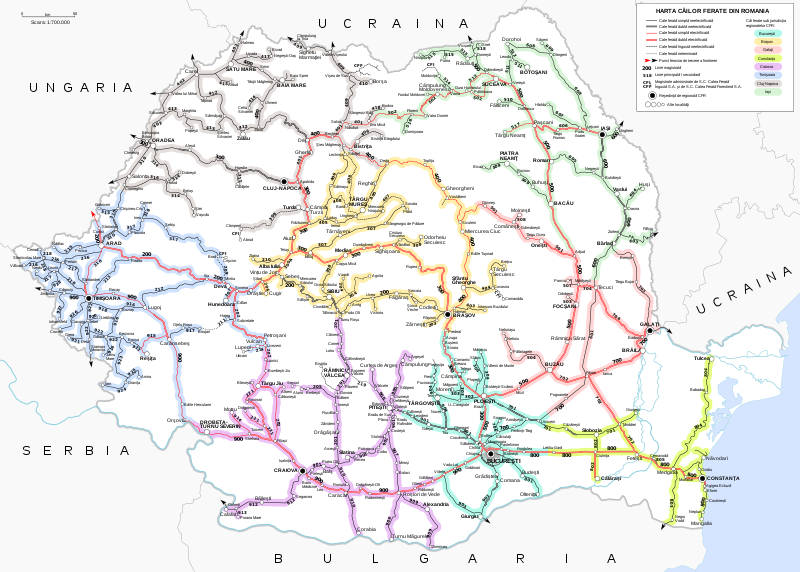
\includegraphics[width=0.8\textwidth]{./figures/ch3_romania-feroviara.png}
    \caption{Map of Romania's railway network. Map by Aero Avalon, shared under CC-BY 4.0 \cite{WikipediaRomaniaFeroviara}.}
    \label{FigRomaniaFeroviara}
\end{figure}

The passenger subsidiary, CFR Călători, is the biggest railway operator that makes use of these lines. However, rolling stock is outdated and most train cars lack modern features like driver-controlled doors. A notable absence though is that of live travel information offered inside the train to the passengers. Examples of such information displays are given in figures \ref{FigMAVInterior}.

\begin{figure}[htbp]
    \centering
    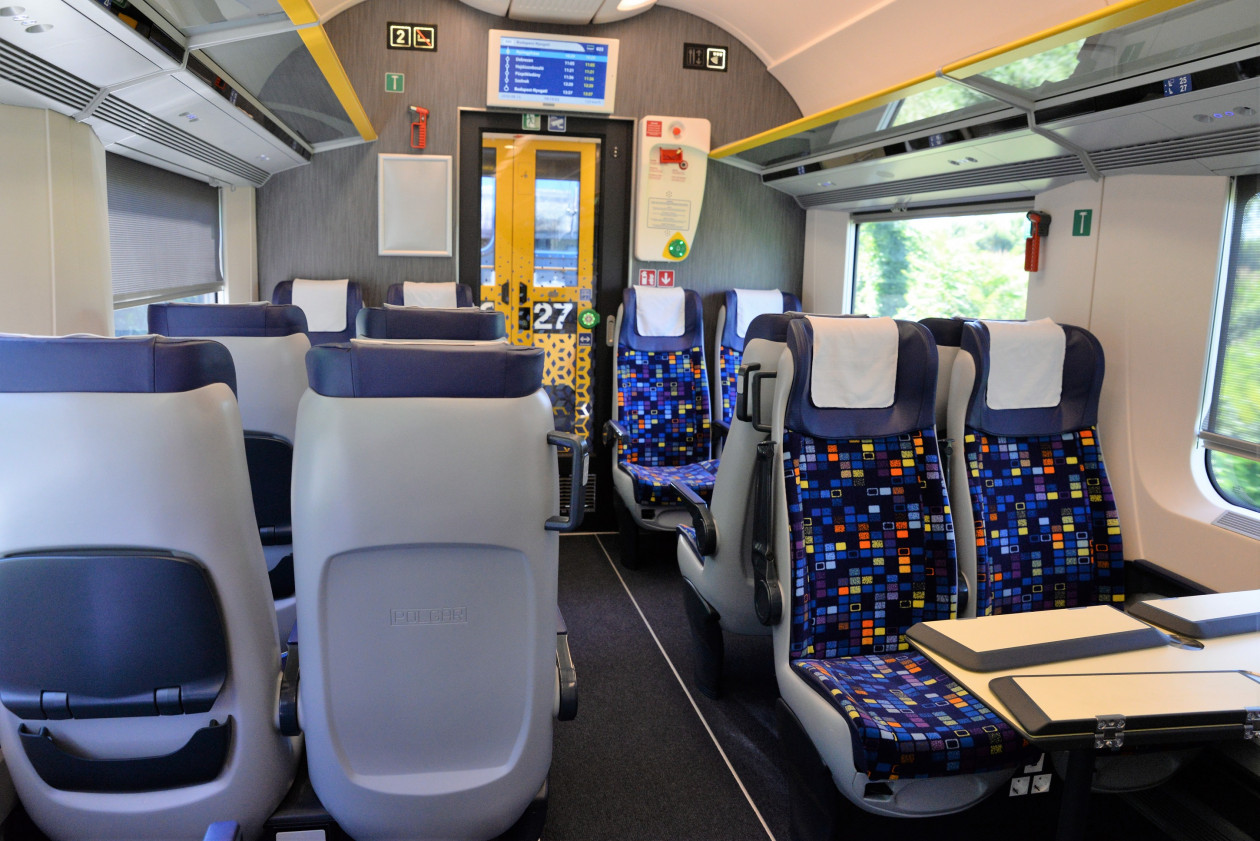
\includegraphics[width=0.8\textwidth]{./figures/ch1_mav-interior.png}
    \caption{Interior of a train owned by MÁV-Start, the Hungarian national passenger operator \cite{PestiHirlapMAVInterior}. The LCD display can be seen at the top, providing information about the next stations, times and delays. Stations and times can be pre-programmed into the train on departure, but delays require live integration with a central service.}
    \label{FigMAVInterior}
\end{figure}

Given that retrofitting all rolling stock with displays connected to the Internet is a challenging task, CFR Călători has attempted digitization in various other ways.

In 2016, the company launched IRIS, a web application that provided traffic information about the company's trains. It also offered information about delays \cite{StiriDeClujLansareCFRIris}. In 2018, IRIS got discontinued in favor of a newer platform, written in ASP.NET, which offers information about all railway operators in Romania.

In 2021, the company launched a mobile application with all the capabilities that the website has, making it more convenient than ever before to view traffic information \cite{MobilissimoCFRLansareMobil}.

These solutions, however, are insufficient in answering the question of "Where am I?" that a passenger might have. The most significant issue is that they all require Internet, the lack of which is an issue prevalent across Romanian trains \cite{CFRInternetIC}.

Moreover, CFR does not track the location of their trains using GPS transponders or any similar technology, but rather using personnel that are responsible with coordinating the trains passing through each station. This brings a number of issues:

\begin{itemize}
    \item \textbf{Data is not real-time.} A train passing through a station is only recorded when the station personnel manually records that train as passed, in the company's internal services.
    \item \textbf{Data might be missing.} Some personnel might not take the time to enter delay data for each passing train.
    \item \textbf{Some stations are not tracked.} Some train stations are big enough to be serviced by regional trains, but not big enough to warrant any personnel responsible with train movement.
    \item \textbf{Data might be false.} Station personnel can enter any delay data they want, having the possibility of hiding delays.
\end{itemize}

\section{Related work}

By having a quick look across Google results for "pwa showcase", one can notice that there exist a number of websites whose sole role is to promote the PWA architecture by showing usage examples of PWA capabilities.

The showcase website created by Joseph Genchik \cite{GenchikPWAShowcase} presents a couple of uses of some phone sensors like Bluetooth, NFC, location, orientation, while also showcasing Web APIs like speech recognition, the Navigator object, web share, WebSockets, and third-party integrations like Auth0 login.

Danny Moerkerke created a website entitled "What PWA Can Do Today" \cite{MoerkerkePWAShowcase} which attempts to be a more feature-complete showcase, making use of diverse Web APIs like shape recognition, barcode detection, protocol handling, notifications API, file system access, storage, background sync, background fetch, payment requests, network information, and speech recognition.

The website at \verb|progressivewebapproom.com| \cite{PWARoom} contains a showcase of a variety of websites and service providers which provide their services using a PWA. Among a multitude of games, notable names include official apps from Tinder, Twitter (now X) and Ride App. It is obvious that these apps are installable due to the fact that the browser gives you the option (sometimes through a pop-up) to install them after first visit.

From looking on the Internet, it is apparent that the PWA architecture is still a novelty among web developers, and used by companies who want to gain some sort of competitive advantage in the user space, by offering varied methods of using their services. In addition, a literature review in the domain of PWAs done by Mole Patrick V. in 2020 \cite{MoleLitRev} suggests that not enough literature exists on the topic of PWAs, and more research is needed around the topic.
